\chapter{Methods\label{cha:methods}}

In this chapter we train a neural network to play the game breakthrough described in 
Chapter \ref{cha:background}. The training process uses MCTS described in Section \ref{sec:mcts} 
to guide it's training.

The training algorithm is a reinforcement learning based self-play algorithm based on the work 
done in AlphaZero (CITE ME).

\subsection{Neural network Architecture}

The neural network architecture we opted to use was a single convolutional layer with a ReLU 
activation function, followed by 5 residual layers, and lastly a split policy/value head.
A figure describing the architecture can be seen in Figure \ref{fig:nnarch}.

\begin{figure}[]
    \centering

    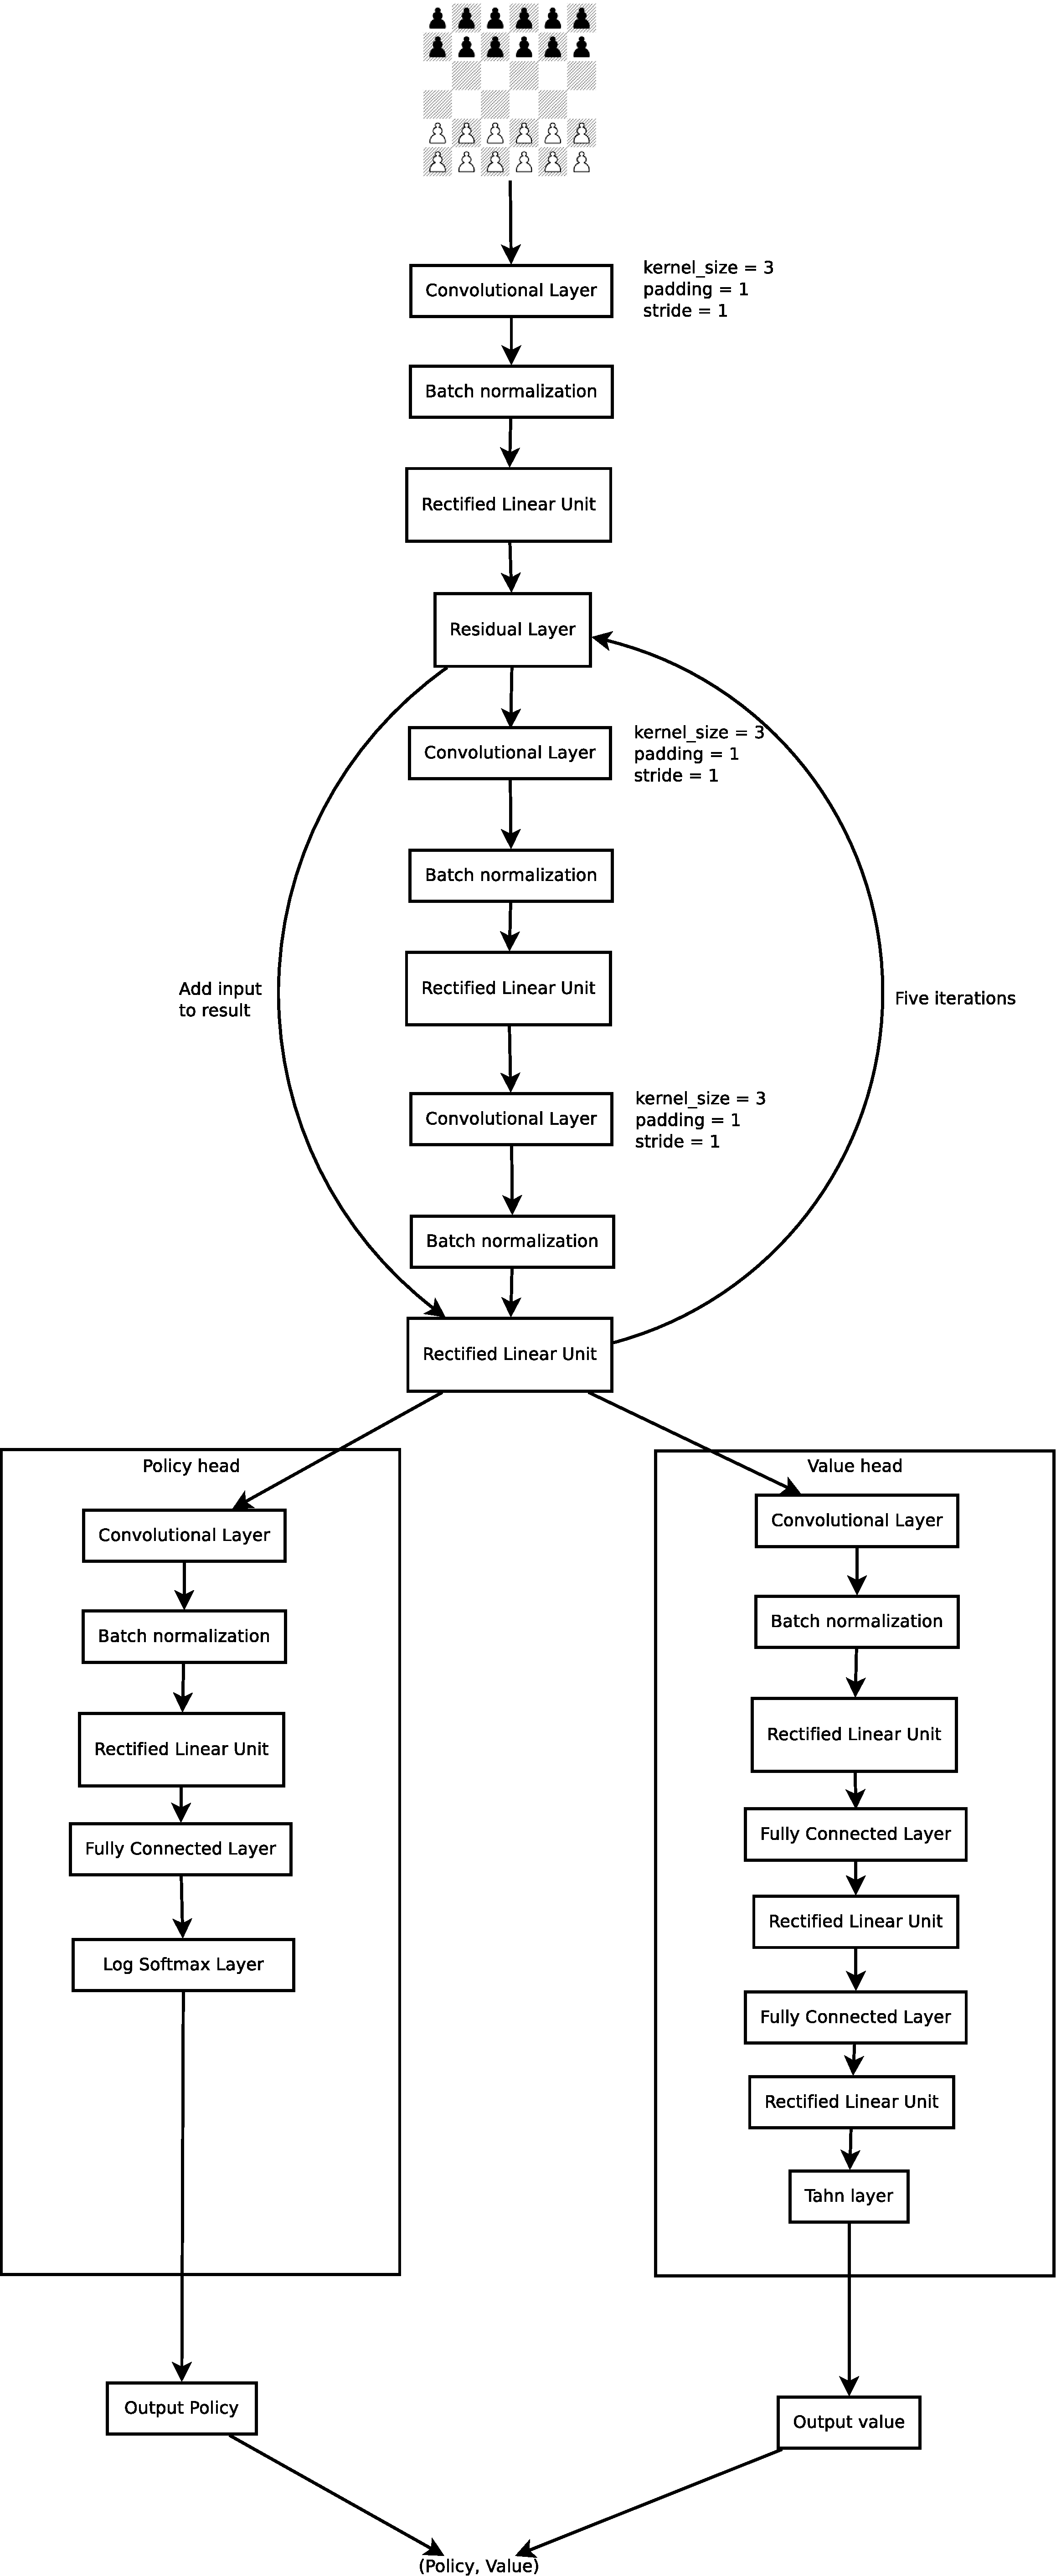
\includegraphics[width=0.65\textwidth]{graphics/test}
    
    \caption{Neural Network Architecture}
    \label{fig:nnarch}
\end{figure}

\subsection{Self-play}

To train the neural network to play Breakthrough we initialize two neural networks $N_1$ and $N_2$ 
with random weights. Then we let $N_1$ play against itself using MCTS to direct its training. 
While playing against itself the neural network gathers data for it to train with. 

The data collected is $(\pi, \tau, p, v)$, where $\pi$ is the action probabilities provided by 
MCTS for $N$ iterations, $\tau$ is the reward for the whole episode, $1$ if white wins,
$-1$ if black wins, and $0$ on a tied game, $p$ is the policy vector
from the neural network, and $v$ is the predicted reward of the game by the neural network.

\subsection{Loss Function}
The data collected is backpropagated through the NN moving the weights to the direction of this 
loss function $l = (p * \pi) + (\tau - v)^2$ for each state the NN encountered during self-play. 